%%%%%%%%%%%%%%%%%%%%%%%%%%%%%%%%%%%%%%
%%%%%%%%%%%%%%%%%%%%%%%%%%%%%%%%%%%%%%
% Do not edit the TeX file your work
% will be overwritten.  Edit the RnW
% file instead.
%%%%%%%%%%%%%%%%%%%%%%%%%%%%%%%%%%%%%%
%%%%%%%%%%%%%%%%%%%%%%%%%%%%%%%%%%%%%%









% \newcommand{\ElectionData}{
% <<graph_fig_cap1>>=
% figcap <- paste(
%     "Some real data. ",
%     "of the IJ and simulation, frequentist error.",
%     sep="")
% SetSlideImageSize(aspect_ratio=1.2, width=0.98)
% @
% <<election_data, cache=knitr_cache, fig.show='hold'>>=
% source(file.path(r_script_dir, "election/data_graph.R"),
%        echo=knitr_debug, print.eval=TRUE)
% @
% }

% The posterior time series prediction is no longer saved.  
% Since time is tight before my presentation, I'm just going 
% to load the old cached results.


\newcommand{\ElectionData}{

\begin{knitrout}
\definecolor{shadecolor}{rgb}{0.969, 0.969, 0.969}\color{fgcolor}

{\centering 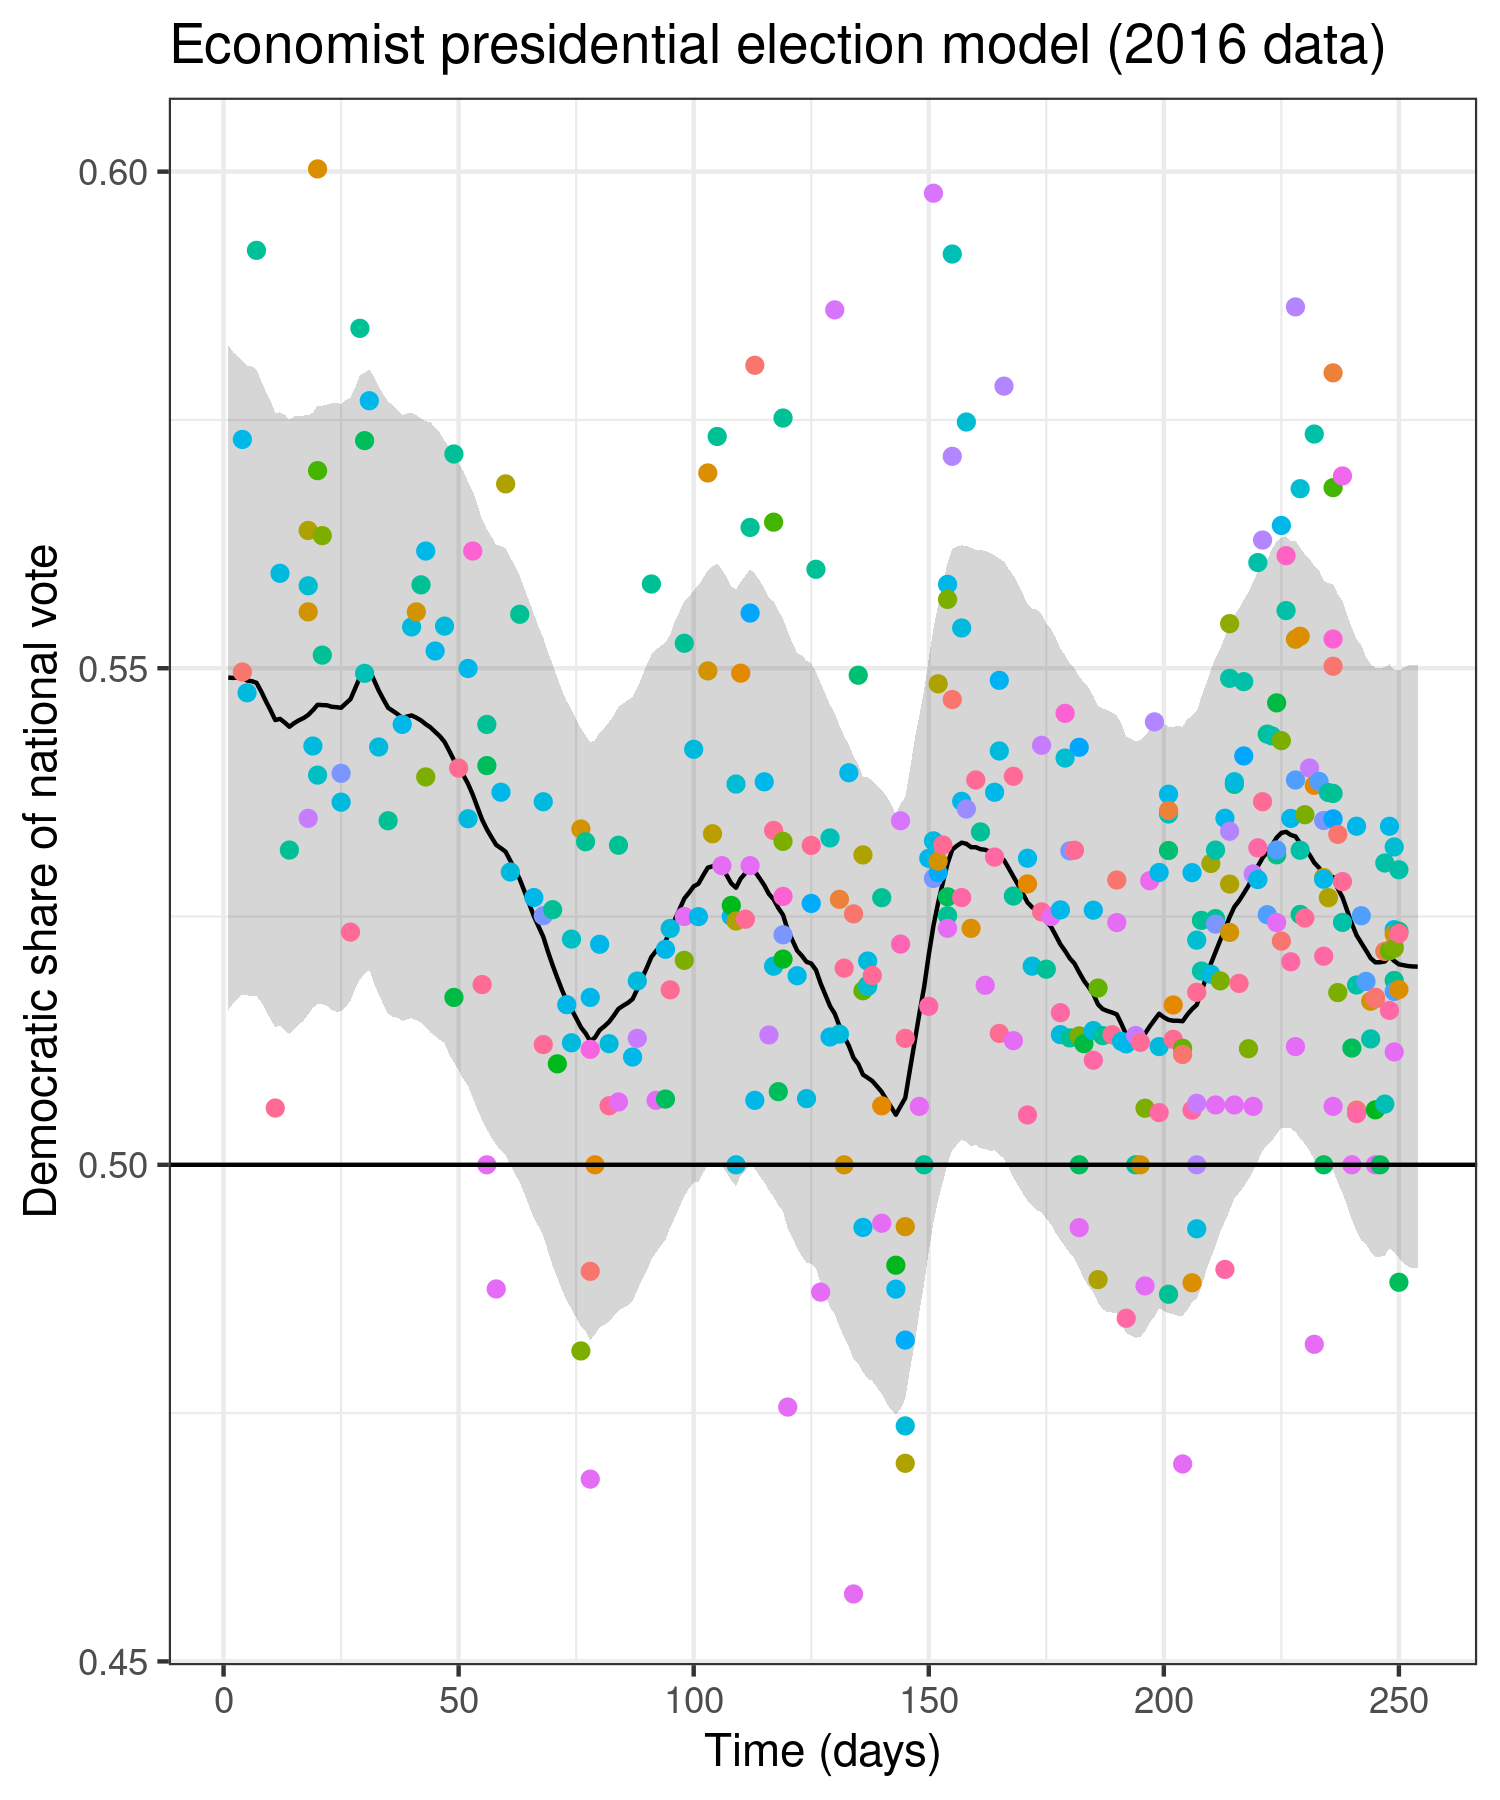
\includegraphics[width=0.980\linewidth,height=1.176\linewidth]{static_figures/election_data-1} 

}



\end{knitrout}
}


\newcommand{\ElectionResultsGlobal}{

\begin{knitrout}
\definecolor{shadecolor}{rgb}{0.969, 0.969, 0.969}\color{fgcolor}

{\centering 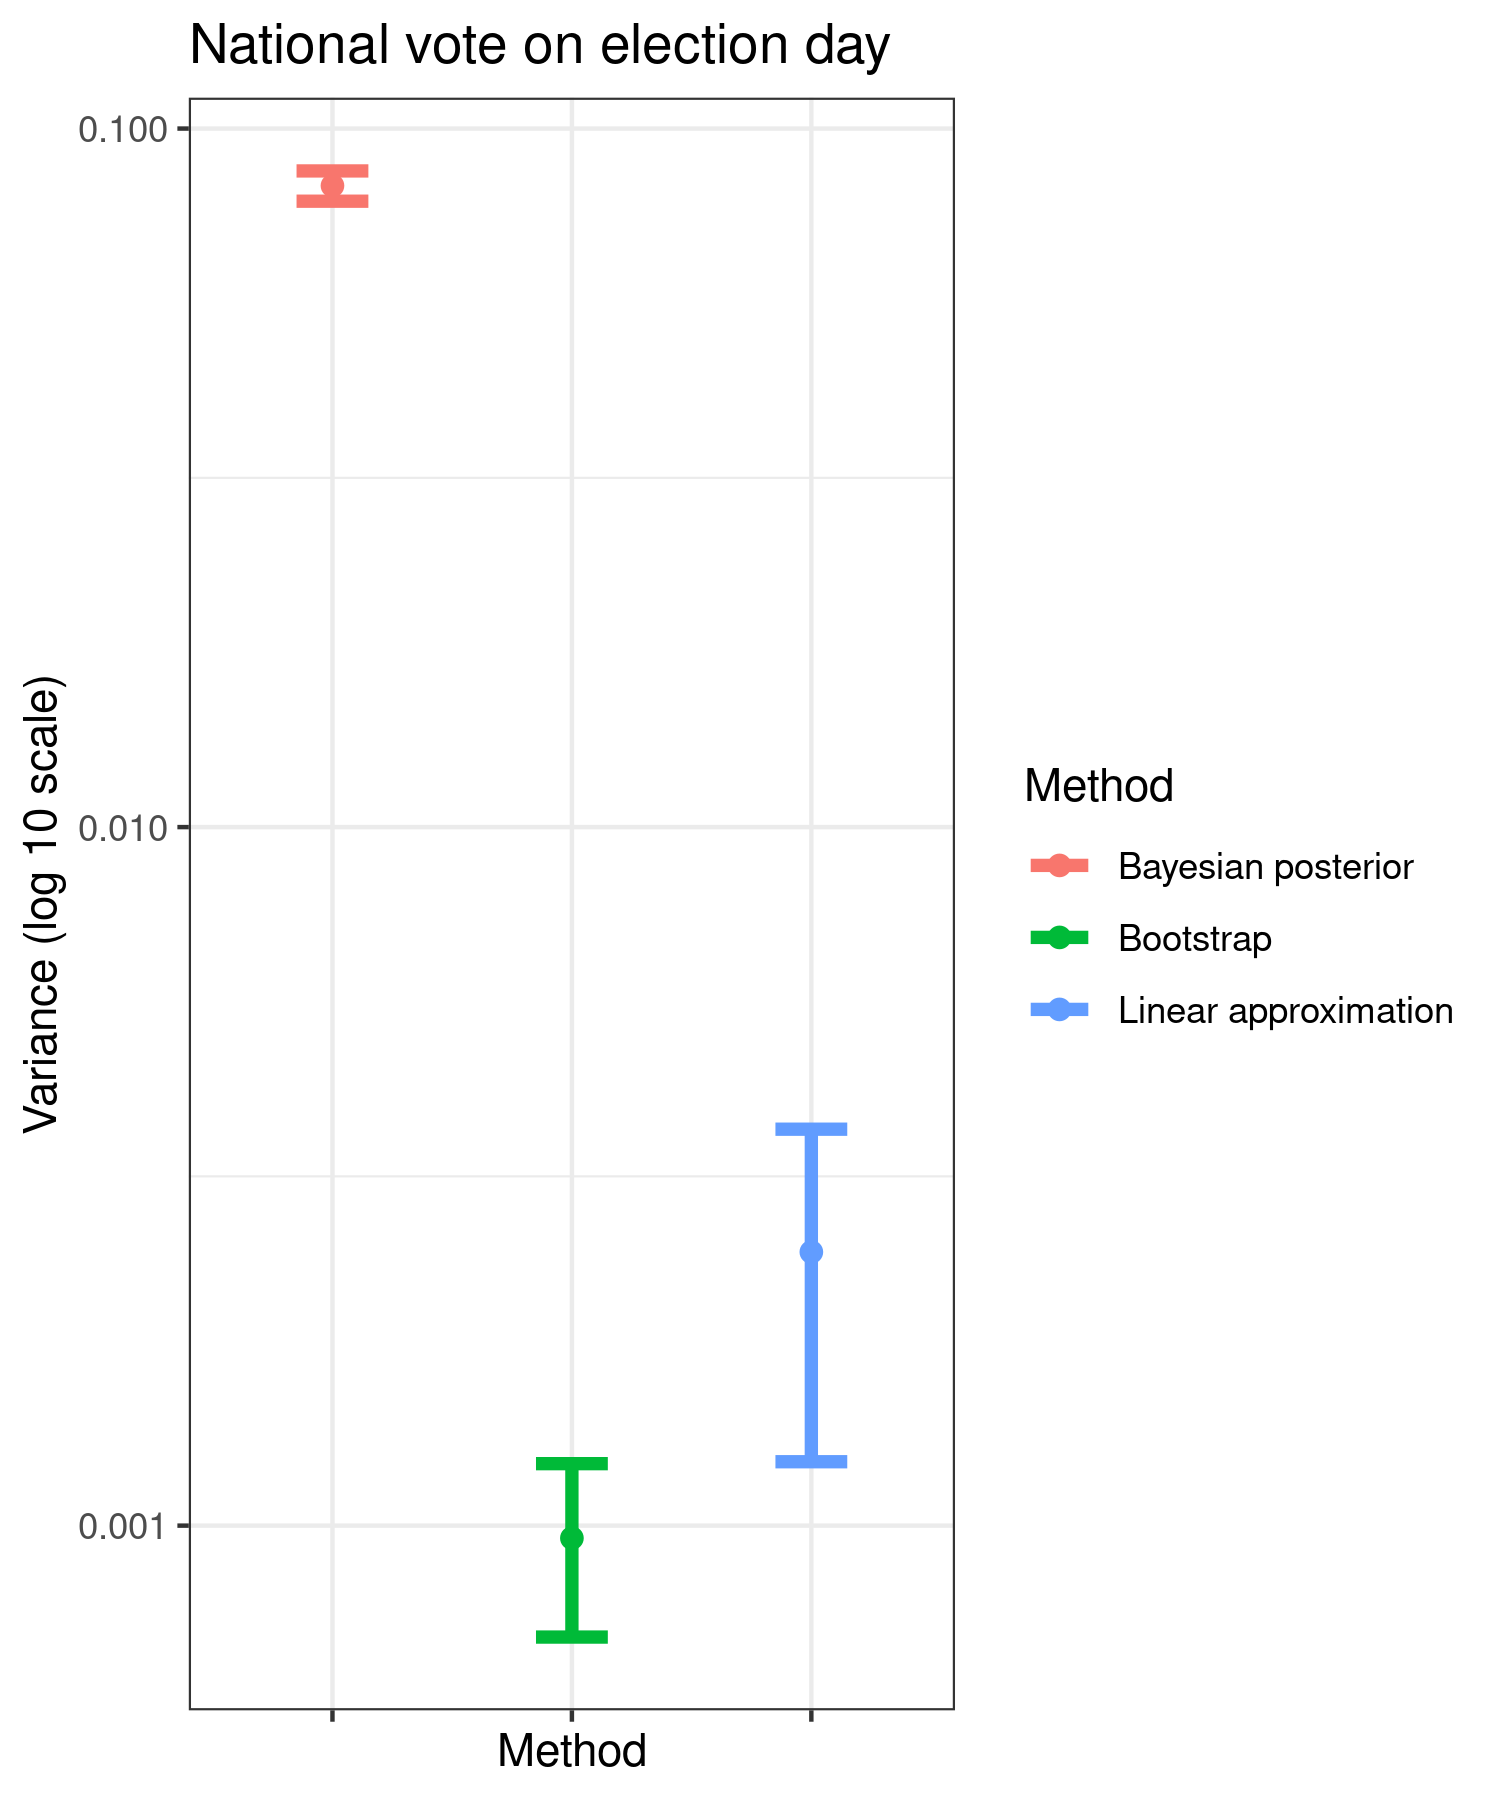
\includegraphics[width=0.980\linewidth,height=1.176\linewidth]{static_figures/election_result-1} 

}



\end{knitrout}
}



% \newcommand{\LowDimAccuracyGraph}{
% %<<mult_path, cache=cache, fig.show='hold', fig.cap=fig_cap>>=
% <<lowdim_accuracy, cache=cache, fig.show='hold'>>=

% bclt_df <- df %>%
%     filter(!as.logical(is_cond), num_obs == num_g)

% num_obs <- 800
% ggplot(bclt_df %>% filter(num_obs == !!num_obs)) +
%     geom_point(aes(x=diff_refit, diff_pred)) +
%     geom_abline(aes(slope=1, intercept=0)) +
%     xlab(TeX("Actual difference in $E\\[\\gamma | X\\]$")) +
%     ylab(TeX("Linear approximation")) +
%     ggtitle(sprintf(paste0(
%         "Negative Binomial model \n",
%         "leaving out single datapoints with N = %d"
%         ), num_obs))
% @
% }



% \newcommand{\HighDimAccuracyGraph}{
% %<<mult_path, cache=cache, fig.show='hold', fig.cap=fig_cap>>=
% <<highdim_accuracy, cache=cache, fig.show='hold'>>=

% nonbclt_df <- df %>%
%     filter(as.logical(is_cond), num_obs == num_g)

% num_obs <- 800
% ggplot(nonbclt_df %>% filter(num_obs == !!num_obs)) +
%     geom_point(aes(x=diff_refit, diff_pred)) +
%     geom_abline(aes(slope=1, intercept=0)) +
%     xlab(TeX("Actual difference in $E\\[\\gamma | X\\]$")) +
%     ylab(TeX("Linear approximation")) +
%     ggtitle(sprintf(paste0(
%         "Poisson random effect model \n",
%         "leaving out single datapoints with N = %d"
%         ), num_obs))
% @
% }




\newcommand{\LowDimAccuracyGraph}{
%<<mult_path, cache=cache, fig.show='hold', fig.cap=fig_cap>>=
\begin{knitrout}
\definecolor{shadecolor}{rgb}{0.969, 0.969, 0.969}\color{fgcolor}

{\centering 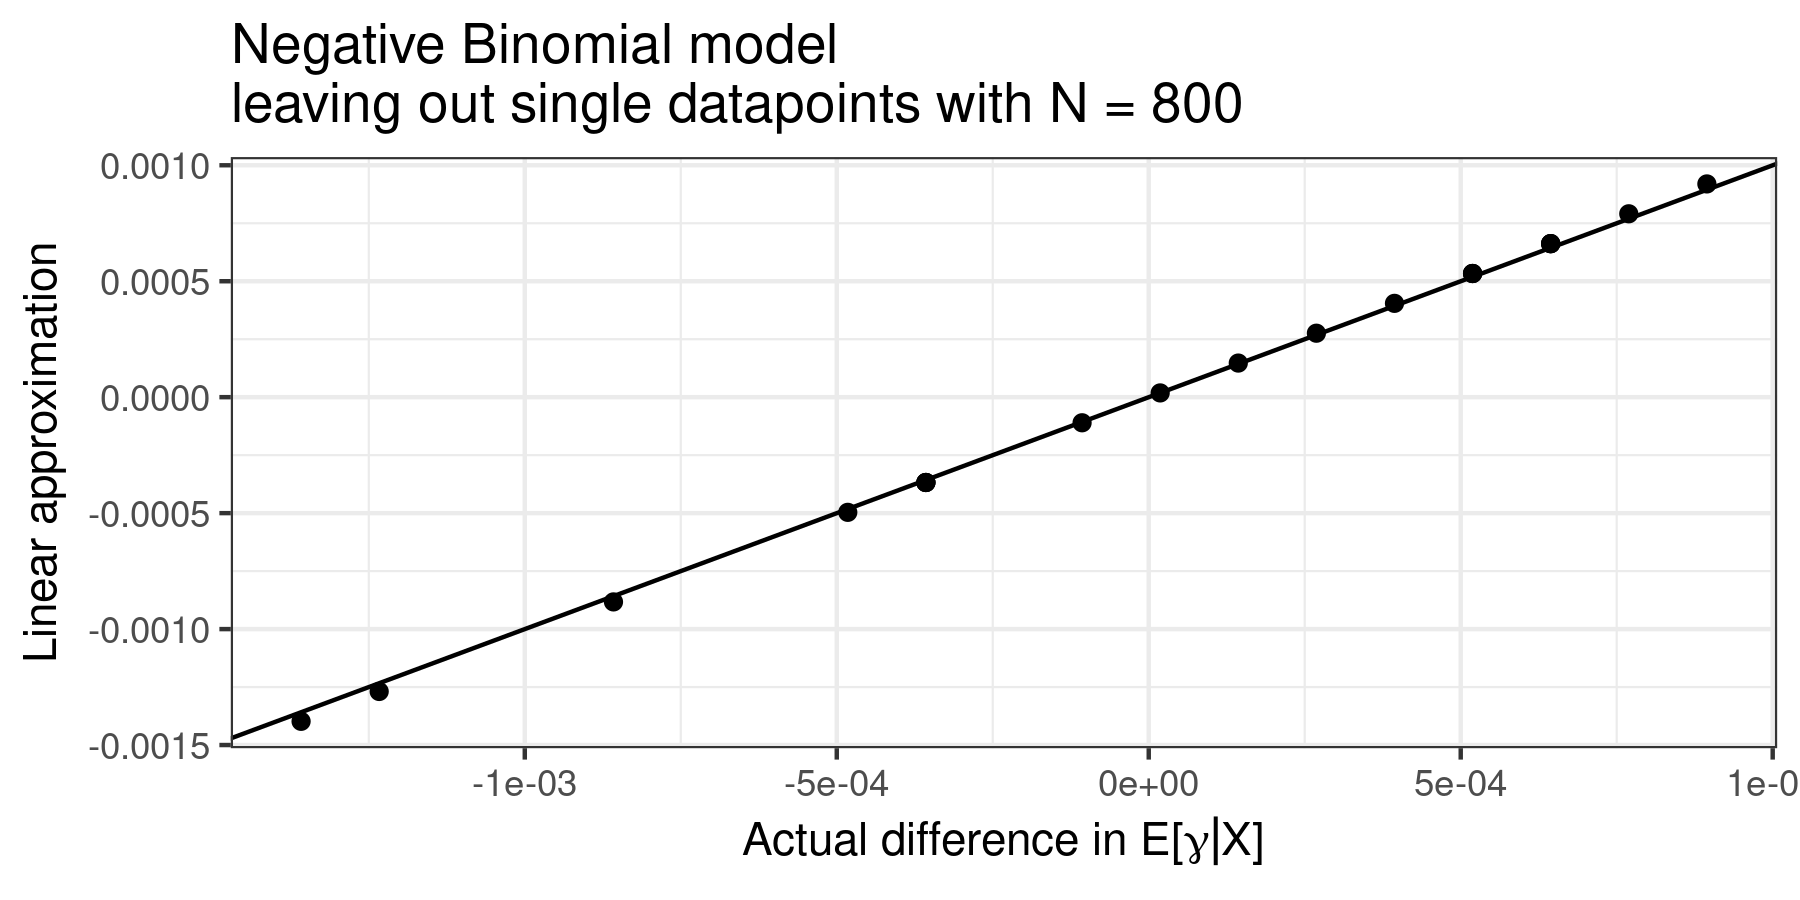
\includegraphics[width=0.980\linewidth,height=0.490\linewidth]{static_figures/lowdim_accuracy-1} 

}



\end{knitrout}
}



\newcommand{\HighDimAccuracyGraph}{
%<<mult_path, cache=cache, fig.show='hold', fig.cap=fig_cap>>=
\begin{knitrout}
\definecolor{shadecolor}{rgb}{0.969, 0.969, 0.969}\color{fgcolor}

{\centering 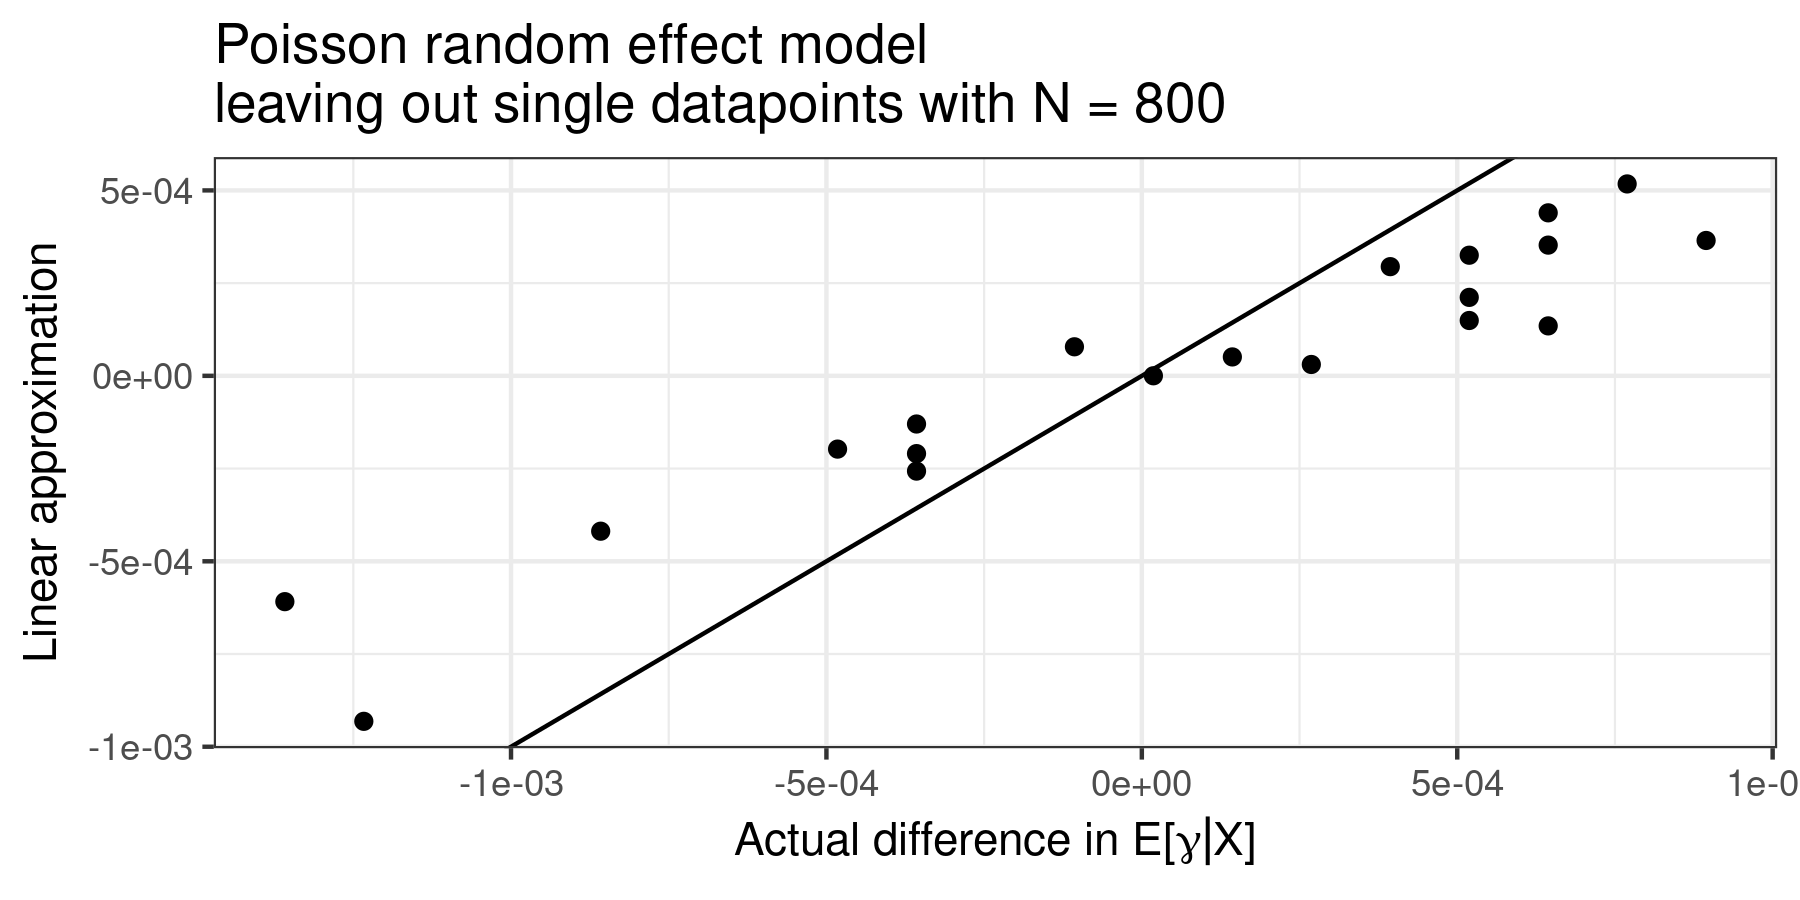
\includegraphics[width=0.980\linewidth,height=0.490\linewidth]{static_figures/highdim_accuracy-1} 

}



\end{knitrout}
}
